\chapter{Formal Analysis Using Alloy}
In this section will be provided a formal model of the problem achieved using Alloy. \\
The model represent only the most important part of the problem, few things have been simplified leaving the more relevant constraints.\newline
For the sake of readability the generated world is split into three sub-worlds which will be explained below.

\section{Alloy Model}
\lstinputlisting[language=alloy]{alloy/model.als}

\subsection{First World}
In the first world (\clupautoref{fig:world1}) the focus is on the \textbf{store} and the \textbf{ticket feature}. The store entity contains all its information, manager and employee user. The store has also a ticket queue which contains only tickets which status is \textit{VALID}.
In case of a ticket \textit{ACTIVE} or \textit{EXPIRED}, the ticket is removed from the queue.
\subsection{Second World}
In the second world (\clupautoref{fig:world2}) the focus is on the \textbf{booking feature}. Store has timeslots which were hidden in the previous world. They represent a slice of time that can be booked.
Every booking must be linked to at least one timeslot. This is because a customer may require to stay in the store longer than just a single timeslot.

\subsection{Third World}
In the third world (\clupautoref{fig:world3}) the focus is on a \textbf{multiple store} implementation. Each store has its information, manager and employee users. It is notable that the CLup admin is \textit{super partes} and has no relation with the number of store.

\begin{figure}[H]
	\centering
	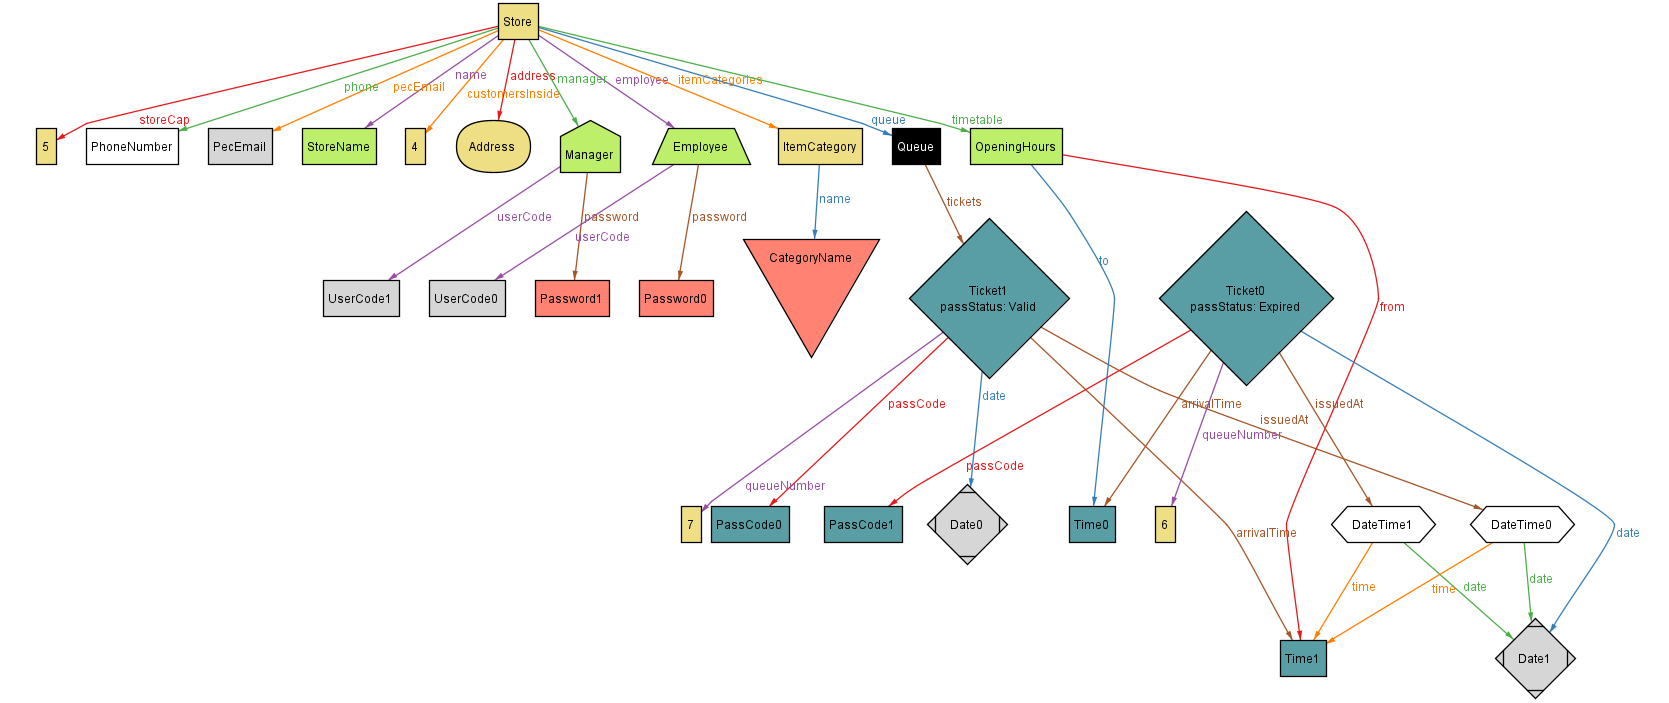
\includegraphics[angle=90,origin=c,height=\textwidth]{world1}
	\caption{First World.}
	\label{fig:world1}
\end{figure}
\begin{figure}[H]
	\centering
	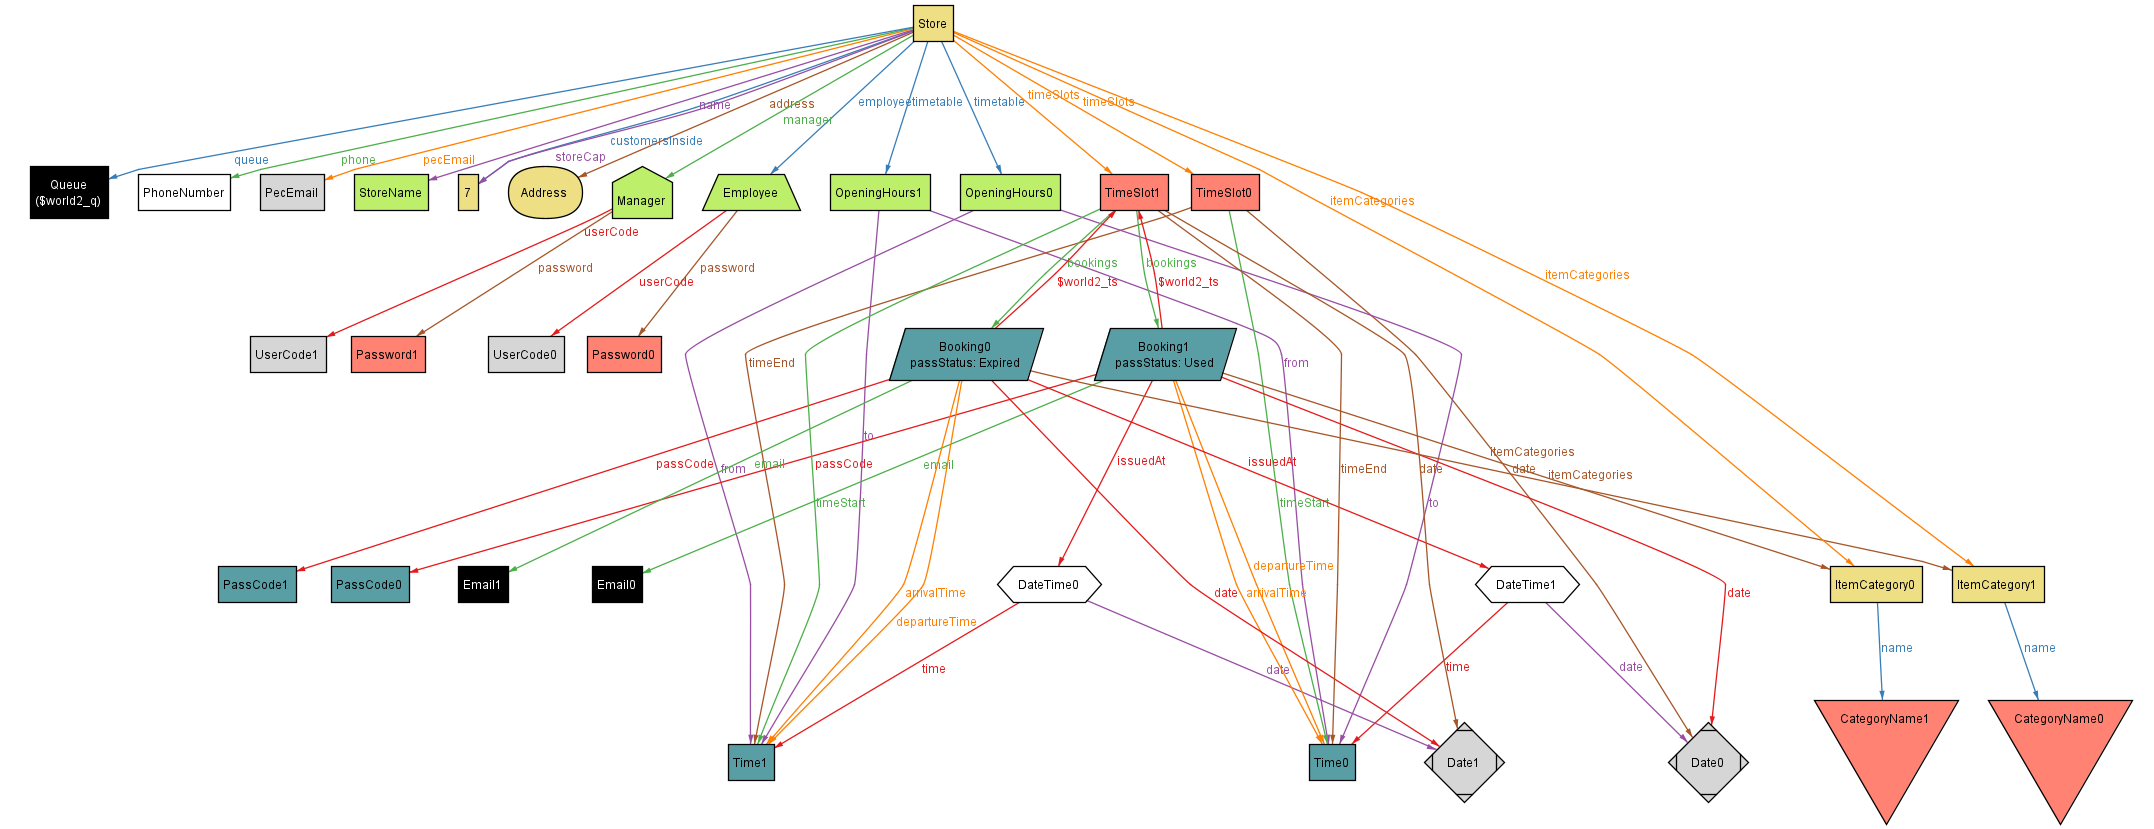
\includegraphics[angle=90,origin=c,height=0.95\textwidth]{world2}
	\caption{Second World.}
	\label{fig:world2}
\end{figure}
\begin{figure}[H]
	\centering
	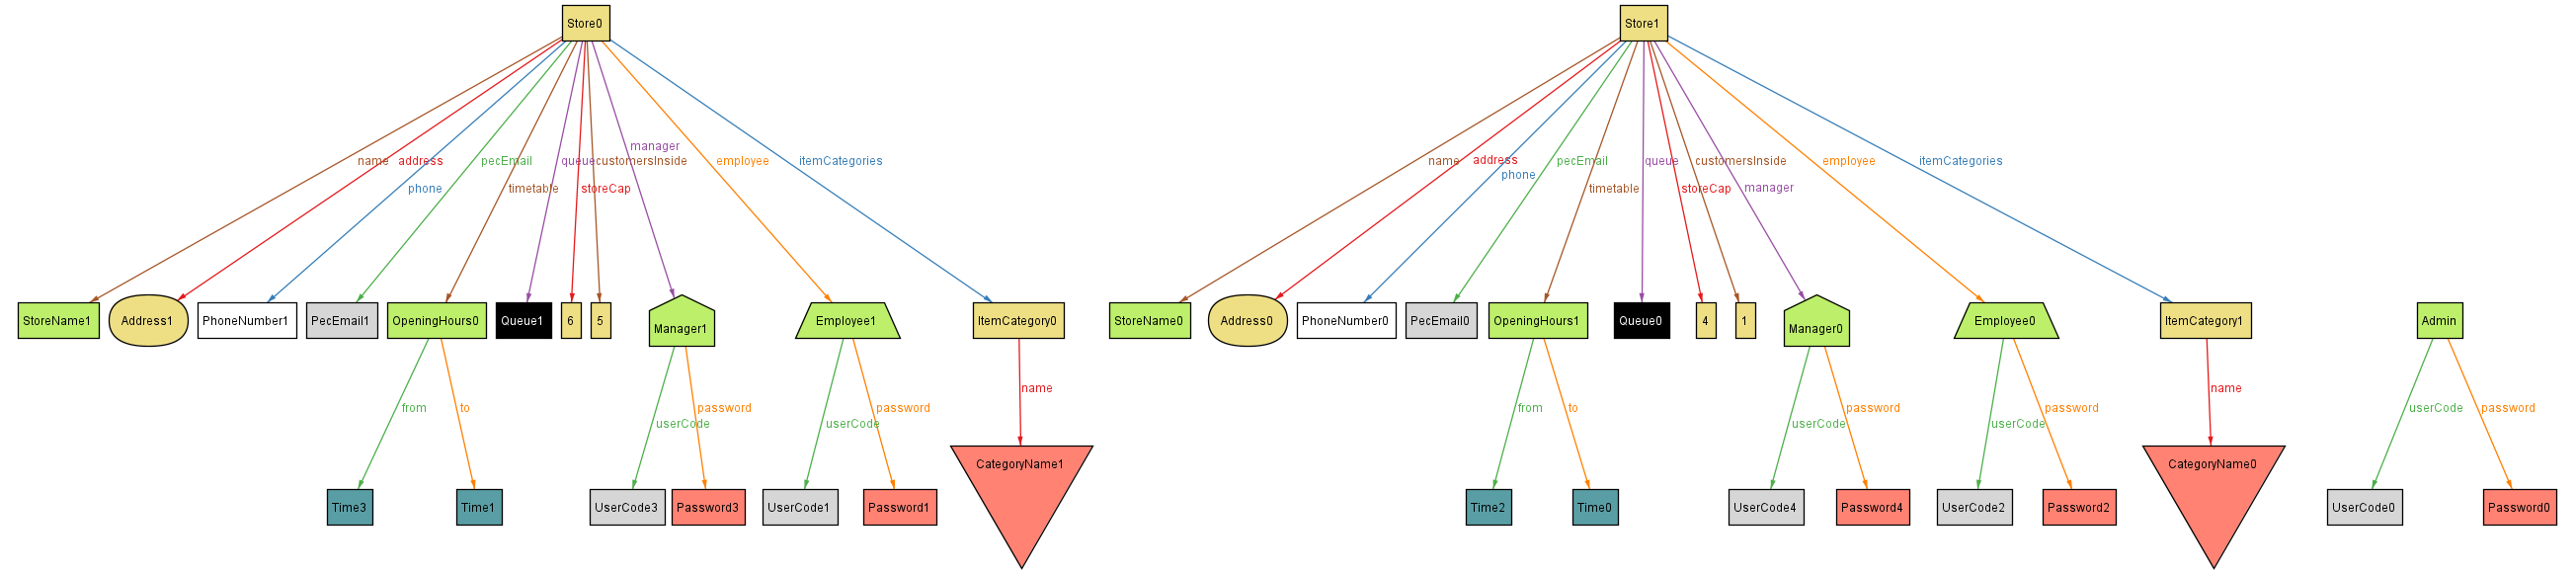
\includegraphics[angle=90,origin=c,height=0.85\textwidth]{world3}
	\caption{Third World.}
	\label{fig:world3}
\end{figure}